\documentclass[11pt]{article}
\usepackage[utf8]{inputenc}
\usepackage{amsmath}
\usepackage[margin=1in]{geometry}
\usepackage{xcolor}
\usepackage{hyperref}
\usepackage{graphicx}

\begin{document}

\newcommand{\Dfrac}[2]{%
  \ooalign{%
    $\genfrac{}{}{1.2pt}0{#1}{#2}$\cr%
    $\color{white}\genfrac{}{}{.4pt}0{\phantom{#1}}{\phantom{#2}}$}%
}
\newcommand{\cond}{\middle\vert}

\section{Table of symbols}
\label{sec:tab-symbols}

\begin{center}
\begin{tabular}{lll}
Symbol & Generation & Meaning\\
\hline
$p$ & $t-1$ & Parental generation\\
$c$ & $t-\frac{1}{2}$ & Contributing (intermediate, selection only)\\
$o$ & $t$ & Offspring (current) generation\\
\end{tabular}
\end{center}

\begin{center}
\begin{tabular}{ll}
Symbol & Meaning\\
\hline
$n$ & Sample size\\
$i$ & Number of derived alleles in sample $n_{\cdot}$\\
$\Dfrac{i}{n}$ & $i$ derived \emph{out of} $n$ total alleles\\
\end{tabular}
\end{center}

\section{Neutral case}

We want to construct the entries in the probability matrix
$P\left[ \Dfrac{\cdot}{n_o} \cond \Dfrac{\cdot}{n_p} \right]$ in terms transition probabilities in
smaller sample sizes. Under neutrality, the number of contributing parental lineages $n'_p$ (at
$t-1$) can not be larger than the number of offspring lineages $n_o$. Since $\mathbf{P}$ is square,
$max(n_p)=max(n_o)=n$. Thus, our aim is to express every entry of $\mathbf{P}$,
$P\left[ \Dfrac{\cdot}{n} \cond\Dfrac{\cdot}{n} \right]$, in terms of
$P\left[ \Dfrac{\cdot}{n-1} \cond \Dfrac{\cdot}{n-1} \right]$. Since we never require extra lineages
($n_p\le n_o$), the recurrence is closed.

To calculate the transition probabilities, we first condition on the state of the last parental
allele drawn, and then on the coalescent event that last offspring lineage participates in. The
recurrence is shown in figure \ref{fig:rec-neutral}. The panel on the right depicts the coalescent
event for each term. Empty circles represent ancestral alleles, filled circles -- derived. The
square box represents a sample of size $n-1$. The first three terms in the sum correspond to the
cases where the last parent that we drew was ancestral, last three -- derived.

\begin{figure}
  \centering
  \includegraphics[width=0.9\textwidth]{fig/recurrence-neutral-annotated.pdf}
  \caption{Recurrence defining transition probabilities in a model without selection. Right panel
    shows coalescent events corresponding to each summand. Each transition probability is defined in
    terms of transition in a smaller sample size. First three terms are conditional on the last
    parent having an ancestral state, last three -- derived. Filled circles -- derived alleles;
    empty circles - ancestral alleles; square brackets -- sample of size $n-1$.}
  \label{fig:rec-neutral}
\end{figure}

When calculating a single entry in \ref{fig:rec-neutral}, the variables have the following ranges.
\begin{equation}
  \begin{aligned}
    n_p &= n \\
    i_p &\in [0, n] \\
    n_o &= n \\
    i_o &\in [0, n] \\
  \end{aligned}
\end{equation}

The recurrence is calculated while $n>1$, with the following base cases:
\begin{align*}
  P\left[ \Dfrac{1}{1} \cond \Dfrac{1}{1} \right] &= 1 \\
  P\left[ \Dfrac{0}{1} \cond \Dfrac{0}{1} \right] &= 1 \\
  P\left[ \Dfrac{0}{1} \cond \Dfrac{1}{1} \right] &= 0 \\
  P\left[ \Dfrac{1}{1} \cond \Dfrac{0}{1} \right] &= 0 \\
\end{align*}

\section{Selection case}

Due to selective deaths, the number of lineages ($n_c$) that contribute to the current generation
can be significantly larger than the number of offspring ($n_o$), and especially so with strong
selection. We use $n_c$, the intermediate number of lineages at time $t-\frac{1}{2}$, which can
potentially be much larger than the number of parents, $n_p$. This is analogous to the gamete
intermediates, as presented in the main text. However, the two are not equivalent, since in this
formulation we apply selection \emph{and} drift on the intermediate lineages. We model the
intermediate contributing alleles as a random sample from $n_p$ alleles, without replacement.

\begin{equation}
  P_s\left[ \Dfrac{i_o}{n} \cond \Dfrac{i_p}{n} \right] = \sum_{i_c,n_c}P_s\left[ \Dfrac{i_o}{n}
    \cond \Dfrac{i_c}{n_c} \right] P_s\left[ \Dfrac{i_c}{n_c} \cond \Dfrac{i_p}{n} \right]
\end{equation}

The probability conditional on the contributing lineages
($P_s\left[ \Dfrac{i_o}{n} \cond \Dfrac{i_c}{n_c} \right]$) is given by equation
\ref{fig:rec-selection}, while $P_s\left[ \Dfrac{i_c}{n_c} \cond \Dfrac{i_p}{n} \right]$ is given by
the hypergeometric distribution. The support of the hypergeometric distribution means that we can
not have $n_c>n$. Note that while $i_c \le n_c \le n$, we can still have $i_c>i_p$ if $i_p$ is
small. A formulation where a $n_c$ is potentially infinitely large will be desirable.

Under the current definition, $P_s$ is not closed, since the cases where $n_c>n$ are not accounted
for. However, as we show in the main text, the formulation is asymptotically closed, as $n$ increases.

The recursive definition in \ref{fig:rec-selection} is analogous to the neutral case, and gives
$P_s\left[ \Dfrac{i_o}{n} \cond \Dfrac{i_c}{n_c} \right]$, the probability that $i_o$ out of $n$
lineages are derived, given that $i_c$ out of $n_c$ contributed to it. To construct this
probability, we condition on the coalescent events involving the last offspring allele. We limit the
model to at most $1$ selective death per lineage. However, in the entire sample, there still can be
a large number of selective deaths. There are 6 distinct coalescent events with $0$ or $1$ selective
deaths, with distinct probabilities based on whether the last offspring allele is ancestral or
derived. This gives 12 different cases:


\begin{figure}
  \centering
  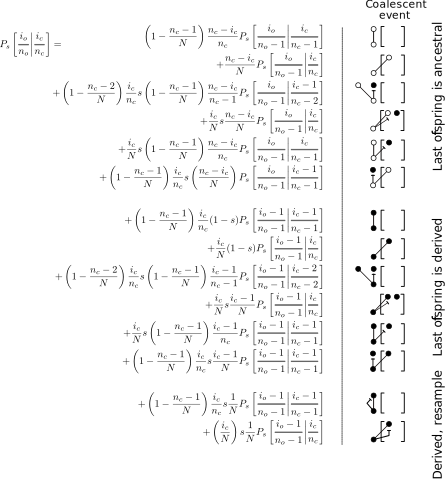
\includegraphics[width=0.9\textwidth]{fig/recurrence-selection-annotated.pdf}
  \caption{Recurrence defining transition probabilities in a model with selection. Right panel
    shows coalescent events corresponding to each summand. Each transition probability is defined in
    terms of transition in a smaller sample size. First six terms are conditional on the last
    offspring having an ancestral state, last six -- derived. Filled circles -- derived alleles;
    empty circles - ancestral alleles; square brackets -- smaller sample.}
  \label{fig:rec-selection}
\end{figure}

For each calculation, the ranges of the variables are:

\begin{equation}
  \begin{aligned}
    n_p &= n \\
    i_p &\in [0, n] \\
    n_c &\in [1, n] \\
    i_c &\in [0, n_c] \\
  \end{aligned}
\end{equation}

Note that unlike in the neutral case $n_c$ is now variable. The base cases of the recurrence are:

\begin{equation*}
  \begin{aligned}
    P\left[ \Dfrac{1}{1} \cond \Dfrac{1}{1} \right] &= 1-s \\
    P\left[ \Dfrac{0}{1} \cond \Dfrac{0}{1} \right] &= 1 \\
    P\left[ \Dfrac{1}{1} \cond \Dfrac{2}{2} \right] &= s \\
    P\left[ \Dfrac{0}{1} \cond \Dfrac{1}{2} \right] &= \frac{1}{s} \\
    \text{otherwise} &\phantom{{}=} 0
  \end{aligned}
\end{equation*}

\end{document}
